% Chapter apnams

\chapter{APNA Management Service} % Main chapter title

\label{apnams} % For referencing the chapter elsewhere, use \ref{apnams}

\section{What is APNA Management Service}
APNA Management Service is responsible for four major tasks primarily:

\begin{itemize}
    \item Ephemeral IDs Management
    \item Domain Name System (DNS)
    \item Message Authentication Key Management
    \item Mapping IPv4/IPv6 addresses to Host Identity
\end{itemize}

\section{Ephemeral IDs Management}
\subsection{Ephemeral ID (EphID) Structure}
We engineered the length of EphID to optimize processing for the AES block cipher as its the only cipher with widespread hardware support, which enables high performance. In order to generate EphIDs we use a CCA-secure encryption scheme. To this end, we use a generic composition called Encrypt-then-MAC that combines a symmetric encryption with a message authentication code (MAC).
Ephemeral IDs are composed of three things:
\begin{itemize}
    \item Initialization vector (IV)
    \item Encrypted Host Identifier (EHID)
    \item Message Authentication Code (MAC)
\end{itemize}

\subsubsection{Initialization Vector (IV)}
Secure operations of this mode in AES requires a unique IV for every encryption operation (i.e. for every EphID)

\subsubsection{Host Identifiers (HID)}
\begin{center}
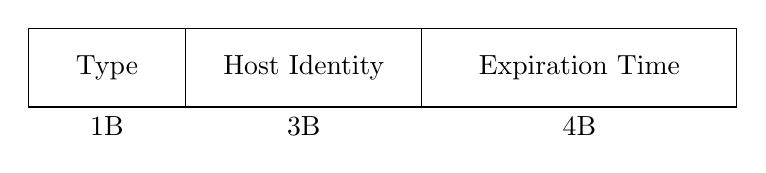
\begin{tikzpicture}
    \draw (0,0) rectangle (2,1) node[pos=.5] {Type}; %node[anchor=north, pos=.5]{0};
    \draw (2,0) rectangle (5,1) node[pos=.5] {Host Identity};
    \draw (5,0) rectangle (9,1) node[pos=.5] {Expiration Time};
    \draw (1 cm,0pt) -- (1 cm,0pt) node[anchor=north] {1B};
    \draw (3.5 cm,0pt) -- (3.5 cm,0pt) node[anchor=north] {3B};
    \draw (7 cm,0pt) -- (7 cm,0pt) node[anchor=north] {4B};
\end{tikzpicture}
\end{center}
Host Identifiers has three main components:
\begin{itemize}
    \item \textbf{Type:} There are two types Control EphID and Session EphID. Control EphID is mainly used to communicate with AS related services. On the other hand Session EphID is used for negotiating a session between client and server. It is also used during the whole communication process.
    \item \textbf{Host Identity:} Host is the 3 byte unique representation for all the host within the AS. It's sufficient enough to uniquely represent all host even in the large ASes.
    \item \textbf{Expiration Time:} This represents the validity of an EphID which is expressed in Unix seconds. Control EphID usually have a longer expiration time than Session EphID. For example in our implementation Control EphID has an expiration time of 1hour and Session EphID has an expiration time of 5mins.
\end{itemize}
\section{Domain Name System (DNS)}
\subsection{Why can't we use current DNS system?}
Since in APNA we replaced IP addresses with Ephemeral Addresses which makes the current DNS system completely obsolete. Currently, DNS only understands how to resolve URL to IP addresses but in order to communicate with other APNA host we would need Ephemeral Address. In order to solve this problem current DNS could be modified be instead of returning A/AAAA records, it could return the certificate associated with the Ephemeral ID. This certificate contains all the details needed to establish the communication between communicating parties.

\subsection{Details}
It's a simple prototype implementation for DNS which works on basic register and request based protocol. For instance a server could register it's associated certificate with DNS when it starts. Whenever a client would need to fetch the server identity it could request from Management Service.

\section{Message Authentication Key Management}
In APNA every packet contains

\section{Mapping IPv4/IPv6 addresses to Host Identity}
Current internet only understands IPv4/IPv6 addresses to route any packet on the internet. In order to route APNA packets we need to build overlay network over the current internet. On other hand we also need 3 bytes unique representation for each host within the AS. So we have used Siphash [??] to create unique 3 bytes representation from IP address.